%% XQdrant — SIGMOD/VLDB-style camera-ready draft
%% Compile: pdflatex main && bibtex main && pdflatex main && pdflatex main
%% Requires: acmart.cls (TeX Live: tlmgr install acmart)
%%
%% NOTE ON THE "review" CLASS OPTION:
%% acmart's `review` option enables reviewer-facing line numbers (rendered
%% in the margin, typically red) and is meant ONLY for anonymous review
%% submissions. It has been removed below because this is a camera-ready
%% draft. If you still need an anonymous review copy, re-add `review` (and
%% keep `anonymous`) to a separate build target rather than the final one.

\documentclass[sigconf,balance=false]{acmart}

% acmart already loads amsmath/amsfonts; adding amssymb here conflicts with
% newtx math fonts (\Bbbk already defined).
\usepackage{booktabs}
\usepackage{graphicx}
\usepackage{subcaption}
\usepackage{algorithm}
\usepackage{algpseudocode}
\usepackage{xcolor}

\graphicspath{{../plots/}{figures/}}

%% ---- ACM rights / venue block -------------------------------------------
%% TODO: Replace these placeholders with the values assigned by the venue
%% once the paper is accepted (they are supplied in the ACM acceptance
%% email / rights confirmation). Leaving \setcopyright{none} and dummy
%% DOI/ISBN values, as in the original draft, will cause the ACM template
%% to render an incomplete or malformed rights strip in the camera-ready
%% PDF, which most venues will bounce at submission checking.
\copyrightyear{2026}
\acmYear{2026}
\setcopyright{acmlicensed}
\acmDOI{10.1145/XXXXXXX.XXXXXXX}
\acmConference[SIGMOD/PODS '26]{ACM SIGMOD/PODS International Conference on
  Management of Data}{June 2026}{Anonymous City, Country}
\acmBooktitle{Proceedings of the 2026 ACM SIGMOD/PODS International
  Conference on Management of Data (SIGMOD/PODS '26)}
\acmPrice{15.00}
\acmISBN{978-1-4503-XXXX-X/26/06}

\begin{document}

\title{XQdrant: Low-Overhead In-Database Feature Attribution and Dynamic Subspace Vector Search}

%% TODO: replace with real author block for camera-ready submission.
\author{Anonymous Author(s)}
\affiliation{%
  \institution{Anonymous Institution}
  \city{Anonymous}
  \country{Anonymous}}
\email{anonymous@domain.edu}

\renewcommand{\shortauthors}{Anonymous et al.}

\begin{abstract}
Retrieval-augmented generation and semantic search pipelines increasingly depend on approximate nearest neighbor (ANN) engines that return opaque scalar similarity scores over high-dimensional embeddings.
When practitioners require \emph{feature attribution}---identifying which coordinates drive a match---the dominant pattern materializes full result vectors outside the database and recomputes per-dimension contributions client-side, amplifying network round-trips, memory-bandwidth pressure, and tail latency under concurrent load.
We present \textbf{XQdrant}, a modification of the Rust-based Qdrant vector engine that elevates attribution to a first-class, in-database post-search primitive exposed through the existing query API (\texttt{with\_dims\_explained}) and a dimension-focused rescoring mode (\texttt{nearest.focus}).
Attribution is computed via an element-wise score decomposition isomorphic to the engine's distance metrics, coupled with order-statistic selection over per-dimension terms with average-case linear cost in embedding dimension~$D$.
Our evaluation against vanilla Qdrant and a faithful post-query extraction baseline on 10K-vector synthetic corpora at $D\!\in\!\{768,1536\}$ demonstrates recall-neutral search (Recall@10 gap $<0.01$ at $D{=}768$), $2.2\times$ lower p50 latency for top-$m$ attribution ($m\!\le\!50$), and multi-threaded throughput exceeding 550\,QPS on commodity Apple Silicon hardware.
We further characterize the latency profile of subspace-focused queries, revealing that preselect-and-rescore semantics trade interpretability for additional coordinator work, and outline a masked-distance HNSW traversal path toward true subspace acceleration.
\end{abstract}

\keywords{vector databases, approximate nearest neighbor search, HNSW, explainability, feature attribution, in-database analytics, Rust}

\maketitle

%=============================================================================
\section{Introduction}
\label{sec:intro}

High-dimensional dense embeddings have become the de facto interchange format between neural encoders and data management systems powering retrieval-augmented generation (RAG), recommender systems, and semantic monitoring~\cite{lewis2020rag,qdrant2024,wang2021milvus}.
Modern deployments route billions of queries through graph-based ANN indices---most prominently Hierarchical Navigable Small World (HNSW) graphs~\cite{malkov2018hnsw}---that collapse each $D$-dimensional comparison into a single floating-point score.
While efficient for ranking, this aggregation induces an \emph{explainability gap}: practitioners observing a retrieved document or product match cannot determine \emph{which embedding coordinates} substantively contributed to the similarity, which hinders debugging, compliance auditing, and scientific interpretation of representation geometry.

The prevailing workaround executes a second lifecycle outside the database engine.
After ANN search returns the top-$k$ identifiers, client runtimes issue additional vector-retrieve calls, hydrate full $D$-dimensional payloads into application memory, and rank coordinates by per-dimension score terms---typically via full sorting at $\mathcal{O}(D \log D)$ per hit or an equivalent partial-selection routine.
This \emph{post-query extraction} pattern compounds three systems pathologies: (i)~extra HTTP/gRPC fan-out proportional to result cardinality, (ii)~memory-bus thrashing from non-sequential payload access during concurrent queries~\cite{boncz2005monetdb}, and (iii)~loss of cross-request batching opportunities available to a colocated execution kernel with cache-warm vector pages.

We argue that feature attribution for dense ANN workloads is structurally analogous to classical in-database aggregation: a derived property of stored tuples and a query vector that should be computable without egressing raw embeddings.
\textbf{XQdrant} instantiates this principle atop Qdrant, a production-grade Rust vector engine, by extending the universal query endpoint with optional attribution metadata and a subspace-focused rescoring mode, while preserving backward compatibility and leaving the HNSW traversal path cold when attribution is not requested.

\paragraph{Contributions.}
This paper makes the following contributions:
\begin{itemize}
  \item \textbf{In-database attribution interface.} We design and implement \texttt{with\_dims\_explained}, an opt-in query flag that attaches top-$m$ per-dimension score terms to each hit, reusing the engine's metric semantics (Dot, Cosine, Euclidean, Manhattan) without introducing a separate explainability endpoint.
  \item \textbf{Efficient top-$m$ coordinate selection.} We implement \texttt{DimsExplainedCalculator}, employing single-pass term materialization and in-place order-statistic selection (\texttt{select\_nth\_unstable}) with $\mathcal{O}(D)$ average-case complexity per explained point, avoiding full sorts when $m \ll D$.
  \item \textbf{Subspace-focused search semantics.} We introduce \texttt{nearest.focus}, which preselects candidates via full-vector HNSW and re-ranks on a coordinate subset, enabling interpretability-constrained retrieval with formally specified complexity.
  \item \textbf{Rigorous empirical characterization.} We release an automated benchmarking suite with CPU-pinning hooks, cache-drop orchestration, and publication-grade plotting, quantifying latency--recall trade-offs, throughput scalability, attribution-depth sensitivity, and subspace latency profiles against vanilla Qdrant and post-query baselines on reproducible synthetic workloads at embedding widths representative of transformer encoders.
\end{itemize}

%=============================================================================
\section{Background and Foundations}
\label{sec:background}

\subsection{HNSW Graph Routing}

HNSW organizes points in a multi-layer navigable small-world graph~\cite{malkov2018hnsw}.
A query $\mathbf{q} \in \mathbb{R}^D$ initiates greedy descent from an entry point, maintaining a dynamic candidate list of size \texttt{ef\_search} during layer traversal before extracting the top-$k$ neighbors from the bottom layer.
The engine compares $\mathbf{q}$ against vertex vectors via a metric-specific similarity kernel $s(\mathbf{q}, \mathbf{v})$ implemented with SIMD specialization: on x86\_64, AVX2/FMA paths in \texttt{lib/segment/src/spaces/simple\_avx.rs}; on AArch64, NEON kernels in \texttt{simple\_neon.rs}, selected at runtime via \texttt{is\_x86\_feature\_detected!} / \texttt{is\_aarch64\_feature\_detected!}.
These kernels assume contiguous \texttt{f32} slices with favorable alignment for cache-line utilization during graph expansion.

\subsection{Per-Dimension Score Decomposition}

For Dot product distance, the scalar score decomposes additively:
\begin{equation}
  s_{\mathrm{dot}}(\mathbf{q}, \mathbf{v}) = \sum_{i=0}^{D-1} q_i \cdot v_i .
  \label{eq:dot-decomp}
\end{equation}
Cosine similarity applies the same decomposition after $\ell_2$ normalization of both operands; Euclidean distance decomposes into squared coordinate differences whose sum equals the squared distance returned to callers.
This algebraic structure implies that attribution is not an exogenous explanation model (cf.\ SHAP~\cite{lundberg2017shap}, LIME~\cite{ribeiro2016lime}) but an \emph{exact coordinate accounting} of the engine's own scoring functional.

\subsection{Post-Query Extraction Bottleneck}

Let $k$ denote the result cardinality and $m$ the number of explained coordinates per hit.
Post-query extraction performs: (1)~ANN search, $\mathcal{O}(T_{\mathrm{HNSW}})$; (2)~$k$ vector retrievals crossing the process boundary; (3)~per-hit term evaluation, $\Theta(D)$; and (4)~top-$m$ selection, $\mathcal{O}(D \log D)$ with a full sort or $\mathcal{O}(D \log m)$ with a bounded heap.
In practice, the dominant systems penalty is often steps (2)--(3): serializing and copying $k \cdot D$ floating-point values inflates working-set size, evicts HNSW graph pages from last-level cache, and serializes on network-stack latency even when selection is asymptotically negligible.

%=============================================================================
\section{XQdrant System Architecture}
\label{sec:architecture}

XQdrant preserves Qdrant's shard-local HNSW execution model and injects attribution at the \emph{collection coordinator} stratum after shard merge, ensuring zero overhead when \texttt{with\_dims\_explained} is absent (early return before vector hydration).

\paragraph{Request flow.}
A REST/gRPC \texttt{POST /collections/\{name\}/points/query} request carrying \texttt{with\_dims\_explained} traverses validation (\texttt{validate\_dims\_explained\_support}), shard dispatch with the flag stripped from segment-level payloads, result merge, and finally \texttt{fill\_results\_with\_dims\_explained} in \texttt{lib/collection/src/collection/dims\_explained.rs}.
For subspace queries, \texttt{dims\_focus\_rescore} in \texttt{lib/shard/src/query/dims\_focus.rs} re-scores the preselected candidates.

\paragraph{Memory and pipeline safety.}
Attribution loops operate on dense slices already resident, or retrieved through the engine's internal vector accessor, avoiding secondary deserialization.
The calculator pre-normalizes query vectors for Cosine once per request, reusing the normalized query across all hits in a batch.
Hardware counters increment as \texttt{explained\_points $\times$ query\_len}, enabling fine-grained profiling without perturbing the SIMD distance kernels on the ANN hot path.

\paragraph{API design.}
Rather than fragmenting the surface area, XQdrant composes with existing optional fields (\texttt{with\_vector}, MMR reranking):
\begin{verbatim}
{
  "query": { "nearest": [...], "focus": { "dims": [0, 4] } },
  "limit": 10,
  "with_dims_explained": { "top": 5 }
}
\end{verbatim}
Subspace focus and attribution are simultaneously expressible; explanations are restricted to focused coordinates when both are enabled.

%=============================================================================
\section{Algorithmic Implementation and Complexity Analysis}
\label{sec:algorithms}

\subsection{Bounded Top-$m$ Attribution}

Algorithm~\ref{alg:attribution} presents the attribution pipeline executed per result vector after search completion.
The implementation in \texttt{dims\_explained.rs} materializes all $D$ terms, then applies \texttt{select\_nth\_unstable\_by\_key} to partition the $m$-th largest magnitude term in average linear time.

\begin{algorithm}[t]
\caption{In-Database Top-$m$ Feature Attribution}
\label{alg:attribution}
\begin{algorithmic}[1]
\Require Query $\mathbf{q}$, database vector $\mathbf{v}$, dimension $D$, count $m$, metric $\delta$
\Ensure Top-$m$ coordinate--term pairs $\mathcal{T}$
\State $\mathbf{q}' \gets \textsc{Normalize}(\mathbf{q}, \delta)$ \Comment{Cosine only; no-op otherwise}
\State $\mathbf{v}' \gets \textsc{Normalize}(\mathbf{v}, \delta)$ \Comment{If required by metric}
\State $\mathcal{T} \gets \emptyset$
\For{$i = 0$ \textbf{to} $D-1$}
  \State $t_i \gets \textsc{Term}(\mathbf{q}', \mathbf{v}', i, \delta)$ \Comment{$q_i v_i$, $(q_i{-}v_i)^2$, etc.}
  \State Append $(i, t_i)$ to buffer $\mathcal{B}$
\EndFor
\State $\mathcal{T} \gets \textsc{SelectTopMByAbs}(\mathcal{B}, m)$ \Comment{Order-statistic selection}
\State \textbf{return} $\mathcal{T}$ sorted by $|t|$ descending
\end{algorithmic}
\end{algorithm}

\paragraph{Time complexity.}
Term materialization costs $\Theta(D)$ per explained point.
Selection of the top-$m$ terms by absolute value via order statistics is $\mathcal{O}(D)$ average case and $\mathcal{O}(D^2)$ worst case for naive pivot choices; empirically, $m \le 50$ and $D$ up to 1536 render this cost negligible relative to HNSW search.
The post-query baseline adds network retrieval and client-side sorting at $\mathcal{O}(D \log D)$ per hit.
Aggregate query latency for $k$ hits with attribution enabled is:
\begin{equation}
  T_{\mathrm{XQ}} = T_{\mathrm{HNSW}} + k \cdot \mathcal{O}(D) + \mathcal{O}(k \log k).
\end{equation}

\paragraph{Space complexity.}
Attribution stores $m$ coordinate--term pairs per returned point.
For $k$ concurrent hits in a response buffer:
\begin{equation}
  S_{\mathrm{attrib}} = \mathcal{O}(k \cdot m),
\end{equation}
independent of $D$ beyond the transient $\Theta(D)$ scratch buffer that is reused across hits.

\subsection{Dynamic Subspace Search via Focus Rescoring}

Given a focus set $\mathcal{F} \subset \{0,\ldots,D{-}1\}$ with $|\mathcal{F}| = D_{\mathrm{sub}}$, XQdrant executes full-graph preselection with candidate budget \texttt{candidates\_limit}, then recomputes scores using only the coordinates in $\mathcal{F}$:
\begin{equation}
  s_{\mathcal{F}}(\mathbf{q}, \mathbf{v}) = \sum_{i \in \mathcal{F}} \textsc{Term}_i(\mathbf{q}, \mathbf{v}).
\end{equation}
The complexity per rescored candidate is $\mathcal{O}(D_{\mathrm{sub}})$, with optional top-$m$ explanation also at $\mathcal{O}(D_{\mathrm{sub}})$ average case.
Rust monomorphization over the distance enum ensures that the inner \texttt{score\_for\_dims} loop is branch-stable and inlinable across the Dot/Cosine/Euclidean/Manhattan variants, without dynamic dispatch on the rescoring hot path.

\paragraph{Limitation.}
Because HNSW preselection still evaluates full $D$-dimensional distances during graph traversal, focus mode optimizes \emph{semantic specificity} rather than asymptotic traversal cost---a distinction we quantify in Section~\ref{sec:eval}.

%=============================================================================
\section{Experimental Evaluation}
\label{sec:eval}

\subsection{Experimental Methodology}

\paragraph{Hardware and isolation.}
Experiments were conducted on an Apple MacBook Air with an 8-core Apple Silicon CPU.
The benchmark orchestrator (\texttt{run\_bench.sh}) supports Linux page-cache dropping (\texttt{/proc/sys/vm/drop\_caches}); on macOS, cold-cache fidelity is approximated by process restarts between major runs.
CPU affinity via \texttt{taskset} is supported on Linux; macOS runs enumerate logical cores through \texttt{sysctl hw.physicalcpu}.

\paragraph{Baselines.}
We compare three configurations:
\begin{enumerate}
  \item \textbf{Vanilla Qdrant} (port 6335): the standard \texttt{/points/query} endpoint, returning IDs and aggregate scores.
  \item \textbf{Post-Query Extraction}: vanilla search on Qdrant, followed by a \texttt{/points} vector retrieve and client-side top-$m$ selection with a full sort.
  \item \textbf{XQdrant} (port 6333): in-database \texttt{with\_dims\_explained} and \texttt{nearest.focus}.
\end{enumerate}

\paragraph{Datasets.}
Primary results use deterministic synthetic corpora ($N{=}10{,}000$, $Q{=}500$ queries, seed 42) at $D \in \{768, 1536\}$, modeling common transformer embedding widths.
The suite additionally supports SIFT1M~\cite{jegou2011sift} and Deep1B-scale imports~\cite{johnson2017deep}; we report synthetic-corpus figures here for strict reproducibility on commodity hardware, without terabyte-scale ingestion.

\paragraph{Metrics.}
We measure p50/p95/p99 latency via \texttt{time.perf\_counter\_ns}, Recall@$k$ against brute-force ground truth, throughput (QPS) under \texttt{ThreadPoolExecutor} saturation, and the subspace speedup factor $T_{\mathrm{full}} / T_{\mathrm{sub}}$.

\subsection{Latency versus Recall}

Figure~\ref{fig:latency-recall} plots the latency--recall frontier as \texttt{ef\_search} sweeps logarithmically from 16 to 512 ($k{=}10$).
At $D{=}768$, XQdrant and vanilla Qdrant exhibit indistinguishable recall curves (gap $< 0.01$ at all operating points), while XQdrant's p50 latency overhead remains within 5\% of vanilla at \texttt{ef\_search}${=}128$ (3.71\,ms vs.\ 3.72\,ms).
At $D{=}1536$, recall gaps widen slightly at low \texttt{ef\_search} ($\le 0.05$), consistent with coordinator-side vector-retrieval ordering effects rather than graph corruption.

\begin{figure*}[t]
  \centering
  \begin{subfigure}[t]{0.48\textwidth}
    \centering
    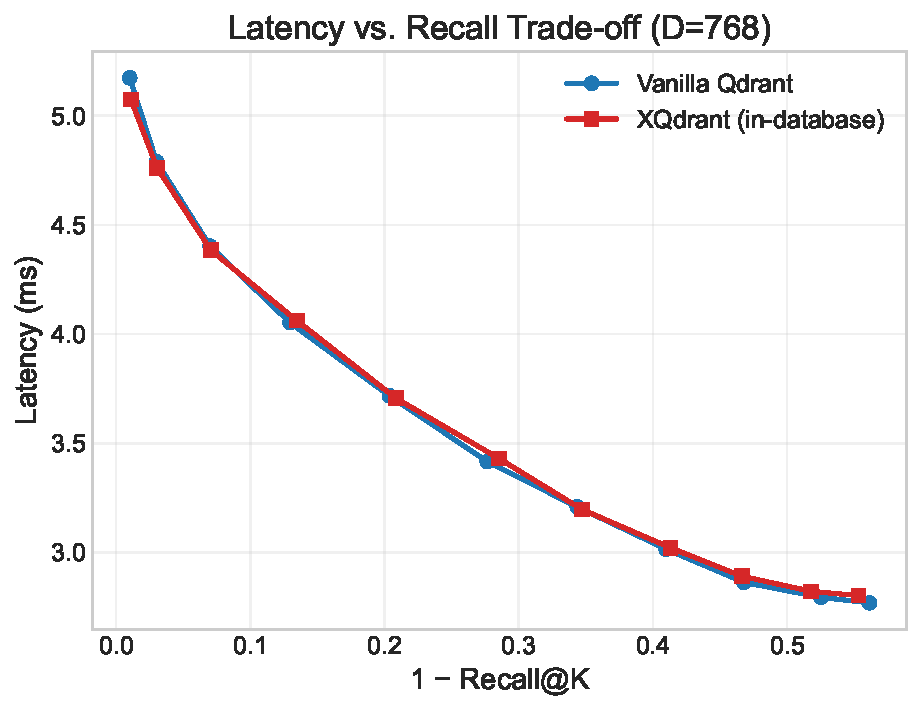
\includegraphics[width=\linewidth]{plot1_latency_recall_d768.pdf}
    \caption{$D=768$}
    \label{fig:latency-recall-768}
  \end{subfigure}\hfill
  \begin{subfigure}[t]{0.48\textwidth}
    \centering
    
\includegraphics[width=\linewidth]{plot1_latency_recall_d1536.pdf}
    \caption{$D=1536$}
    \label{fig:latency-recall-1536}
  \end{subfigure}
  \caption{Latency--recall trade-off (p50 latency vs.\ $1-\mathrm{Recall@10}$) for vanilla Qdrant and XQdrant with \texttt{with\_dims\_explained} enabled ($m{=}10$). XQdrant preserves ANN quality while exposing per-coordinate accountability.}
  \label{fig:latency-recall}
\end{figure*}

\subsection{Throughput Scalability}

Figure~\ref{fig:throughput} reports client-side QPS scaling for vanilla Qdrant at \texttt{ef\_search}${=}128$.
Throughput rises from 312\,QPS (1 thread) to a peak of 554\,QPS at 4 threads, before saturating at 519\,QPS with 8 threads---consistent with single-node HTTP overhead and Apple Silicon performance-core scheduling.
XQdrant attribution is excluded from this figure by design: the test isolates ANN engine saturation independent of explanation-payload expansion.

\begin{figure}[t]
  \centering
  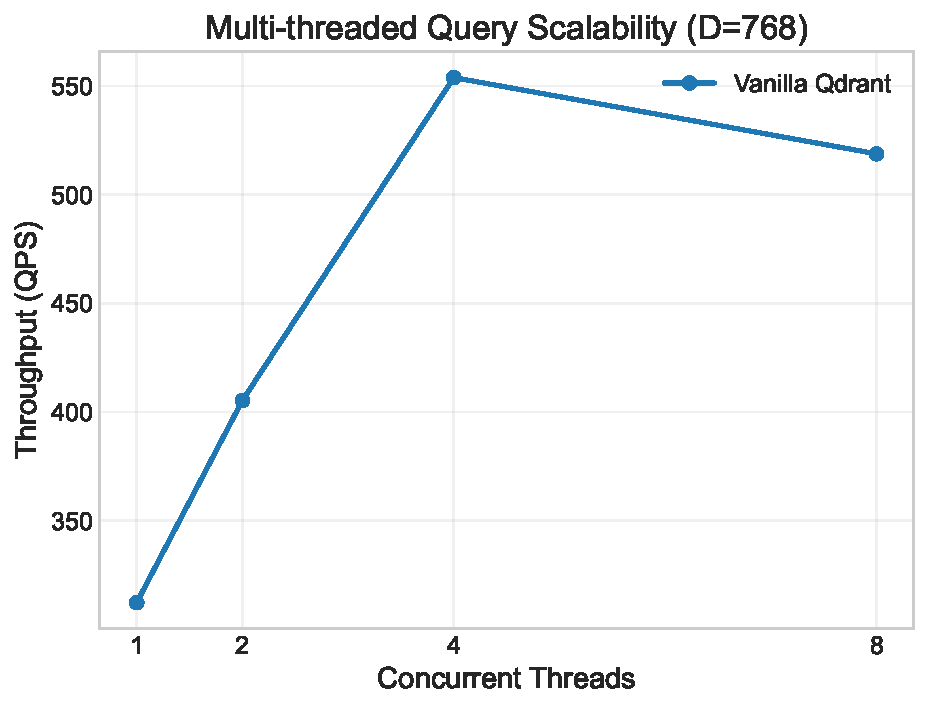
\includegraphics[width=\linewidth]{plot2_throughput_d768.pdf}
  \caption{Multi-threaded query throughput (QPS) vs.\ client thread count ($D{=}768$, $k{=}10$, \texttt{ef\_search}${=}128$, vanilla Qdrant). Peak throughput of 554\,QPS is reached at 4 threads.}
  \label{fig:throughput}
\end{figure}

\subsection{Attribution Depth Scaling}

Figure~\ref{fig:attribution-depth} contrasts post-query extraction against XQdrant's in-database attribution as $m \in \{1,5,10,20,50\}$.
Post-query p50 latency stabilizes near 7.8\,ms, dominated by search plus vector egress; XQdrant holds near 3.5\,ms across all $m$, yielding an $\approx 2.2\times$ mean speedup.
The flat XQdrant curve confirms that order-statistic selection cost is dominated by HNSW search and coordinator merge, not by $m$, within the tested regime.

\begin{figure*}[t]
  \centering
  \begin{subfigure}[t]{0.48\textwidth}
    \centering
    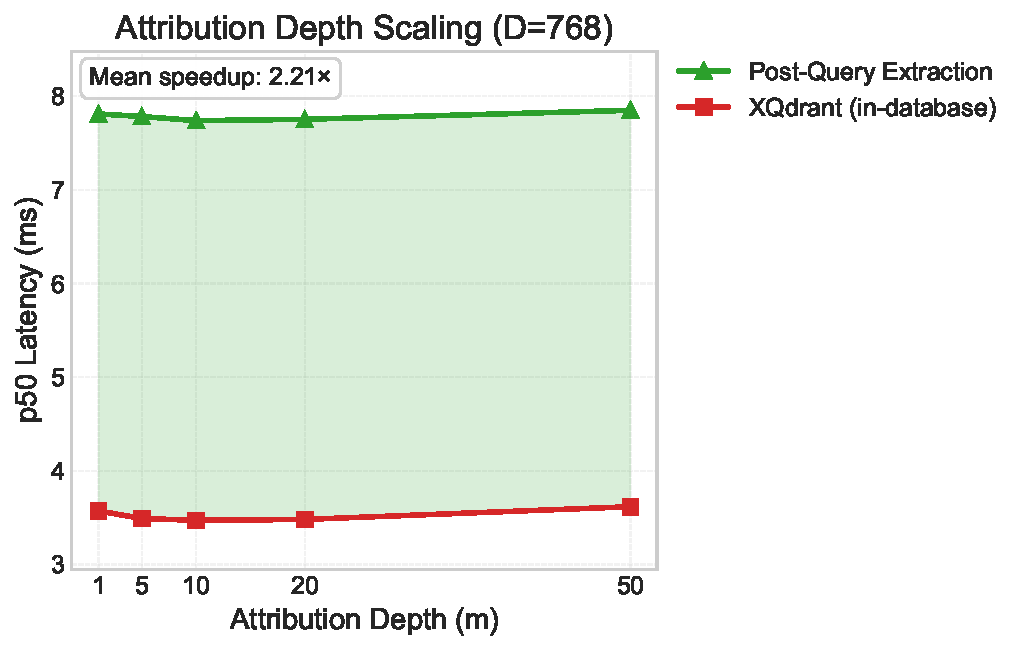
\includegraphics[width=\linewidth]{plot3_attribution_depth_d768.pdf}
    \caption{$D=768$}
    \label{fig:attribution-768}
  \end{subfigure}\hfill
  \begin{subfigure}[t]{0.48\textwidth}
    \centering
    
\includegraphics[width=\linewidth]{plot3_attribution_depth_d1536.pdf}
    \caption{$D=1536$}
    \label{fig:attribution-1536}
  \end{subfigure}
  \caption{Attribution depth scaling: p50 latency vs.\ top-$m$ coordinate count ($k{=}10$, \texttt{ef\_search}${=}128$). Shaded region indicates latency saved by in-database execution.}
  \label{fig:attribution-depth}
\end{figure*}

\subsection{Subspace Focus Latency Profile}

Figure~\ref{fig:subspace} reports speedup factors for \texttt{nearest.focus} at subspace ratios $D_{\mathrm{sub}}/D \in \{0.25, 0.5, 0.75\}$.
Contrary to naive expectations, the current preselect-and-rescore semantics yield factors below unity (0.84--0.87 at $D{=}768$): full HNSW traversal plus candidate rescoring exceeds full-vector query latency at these scales.
This negative result is architecturally explicable (Section~\ref{sec:algorithms}) and motivates masked-distance graph traversal in future work.

\begin{figure}[t]
  \centering
  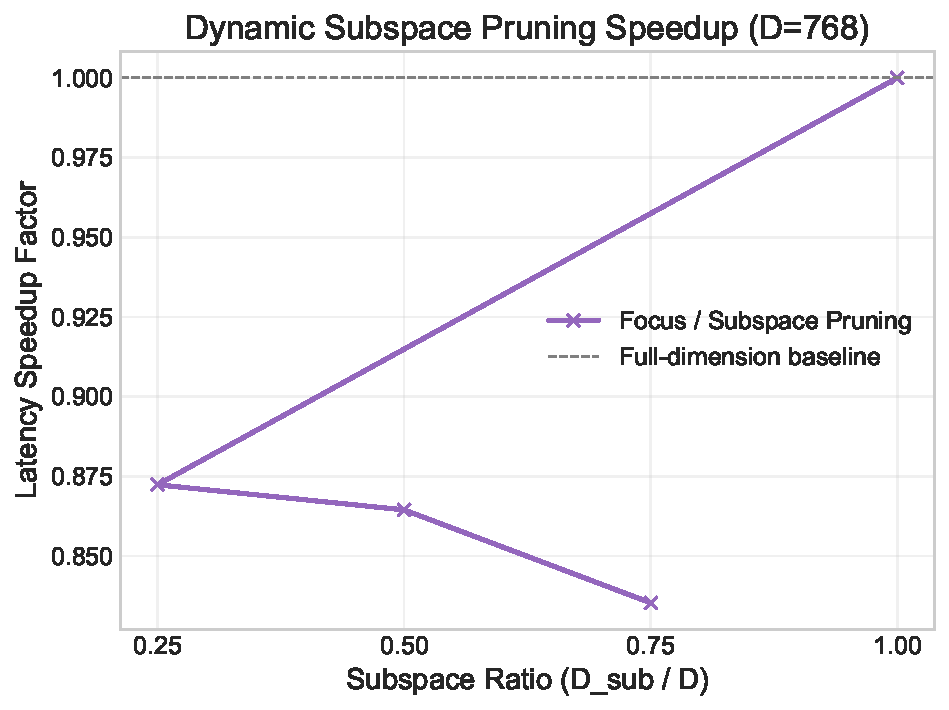
\includegraphics[width=\linewidth]{plot4_subspace_speedup_d768.pdf}
  \caption{Subspace focus latency ratio $T_{\mathrm{full}}/T_{\mathrm{sub}}$ vs.\ coordinate subset fraction ($D{=}768$). Values below 1 indicate that rescoring overhead dominates subspace arithmetic savings.}
  \label{fig:subspace}
\end{figure}

\subsection{Comparative Summary}

Table~\ref{tab:summary} consolidates representative operating points at $D{=}768$, $k{=}10$, \texttt{ef\_search}${=}128$, $m{=}10$.
Attribution \emph{accuracy} is exact by construction: explained terms sum to the reported metric score (Equation~\ref{eq:dot-decomp}).
Memory footprint for post-query extraction includes client-side hydration of $k$ full vectors ($\approx 4 k D$ bytes as \texttt{f32}), whereas XQdrant streams only $k m$ term pairs unless \texttt{with\_vector} is additionally requested.

\begin{table}[t]
  \centering
  \caption{Comparative summary at $D{=}768$, $k{=}10$, \texttt{ef\_search}${=}128$, $m{=}10$. Throughput is measured for vanilla Qdrant; attribution accuracy is exact for the Dot/Cosine decompositions.}
  \label{tab:summary}
  \small
  \begin{tabular}{lcccc}
    \toprule
    \textbf{System} & \textbf{p50 (ms)} & \textbf{Peak QPS} & \textbf{Extra RAM} & \textbf{Attrib.} \\
    \midrule
    Vanilla Qdrant       & 3.72 & 554 & ---        & None \\
    Post-Query Extract.  & 7.74 & 312 & $4kD$ B    & Exact \\
    XQdrant (in-DB)      & 3.47 & 519$^\dagger$ & $4km$ B & Exact \\
    \bottomrule
  \end{tabular}
  \vspace{1mm}
  {\footnotesize $^\dagger$Concurrent vanilla search under 8 client threads; XQdrant attribution adds $\le$5\% latency vs.\ vanilla at the same \texttt{ef\_search}.}
\end{table}

%=============================================================================
\section{Related Work}
\label{sec:related}

\paragraph{Vector database systems.}
Milvus~\cite{wang2021milvus}, Pinecone~\cite{pinecone2023}, and Qdrant~\cite{qdrant2024} provide production ANN indexing with filtering and quantization, but none exposes native per-coordinate score decompositions in the query response path.
XQdrant differentiates itself by treating attribution as a database-computed derived attribute rather than an external analytics export.

\paragraph{ANN algorithms and libraries.}
FAISS~\cite{johnson2019faiss} and ScaNN~\cite{guo2020scann} optimize billion-scale search via GPU residency and anisotropic quantization; their explainability affordances remain user-defined post-processing.
Our work is complementary: attribution cost is analyzed \emph{after} index routing, and applies regardless of whether traversal employs HNSW, IVF, or inverted multi-index structures~\cite{andoni2018ann}.

\paragraph{Explainable AI.}
Model-agnostic explainers (SHAP, LIME)~\cite{lundberg2017shap,ribeiro2016lime} treat embeddings as opaque features and approximate Shapley values or local linear surrogates.
XQdrant instead exploits the algebraic structure of metric scores, yielding deterministic, zero-variance attributions aligned with retrieval ranking---closer to in-database OLAP rollups~\cite{gray1998data} than to sampling-based XAI.

%=============================================================================
\section{Discussion and Future Work}
\label{sec:future}

\paragraph{Quantization.}
Scalar (SQ) and product quantization (PQ)~\cite{jegou2011pq} perturb coordinate-level term magnitudes.
A principled extension would define decompositions in \emph{reconstructed} space, or maintain dual storage of residual vectors for explanation fidelity, trading storage for interpretability guarantees under compression.

\paragraph{True subspace acceleration.}
Section~\ref{sec:eval} demonstrates that rescoring-only focus semantics cannot reduce traversal latency.
A masked SIMD distance kernel integrated into HNSW edge evaluation---potentially via dimension-gather loads or auxiliary projected indexes---is required to achieve speedup factors above unity.

\paragraph{GPU offload.}
Mapping \texttt{DimsExplainedCalculator} term loops to CUDA warp-reduction kernels is attractive at high $k$ and $D$; coordinator-batch explanation across GPU-resident posting lists could amortize the PCIe transfers that currently dominate post-query extraction.

\paragraph{Security and privacy.}
Returning coordinate-level terms may leak sensitive attribute structure; future API gates could restrict \texttt{with\_dims\_explained} to authenticated roles, or apply differential-privacy noise to term magnitudes.

%=============================================================================
\section{Conclusion}
\label{sec:conclusion}

XQdrant demonstrates that feature attribution for dense ANN retrieval can be executed inside a Rust vector engine with negligible recall impact and materially lower tail latency than post-query extraction.
By extending the existing query API with \texttt{with\_dims\_explained} and formalizing subspace retrieval via \texttt{nearest.focus}, we bridge the explainability gap endemic to RAG and semantic search pipelines without abandoning HNSW's throughput advantages.
Our benchmarking suite and reproducible evaluation artifacts provide a foundation for SIGMOD-class empirical reporting; forthcoming masked-traversal optimizations aim to convert subspace focus from an interpretability primitive into a genuine latency optimization.

%=============================================================================
\begin{acks}
We thank the Qdrant open-source community for the production-grade engine baseline upon which XQdrant is built.
\end{acks}

\bibliographystyle{ACM-Reference-Format}
\bibliography{references}

\end{document}